% PPO actor-critic MLP architecture
% Compile with: pdflatex arch_ppo.tex
\documentclass[tikz,border=2pt]{standalone}
\usepackage{amsmath}
\usetikzlibrary{arrows.meta,positioning,shapes.geometric,fit,backgrounds,calc}

\begin{document}
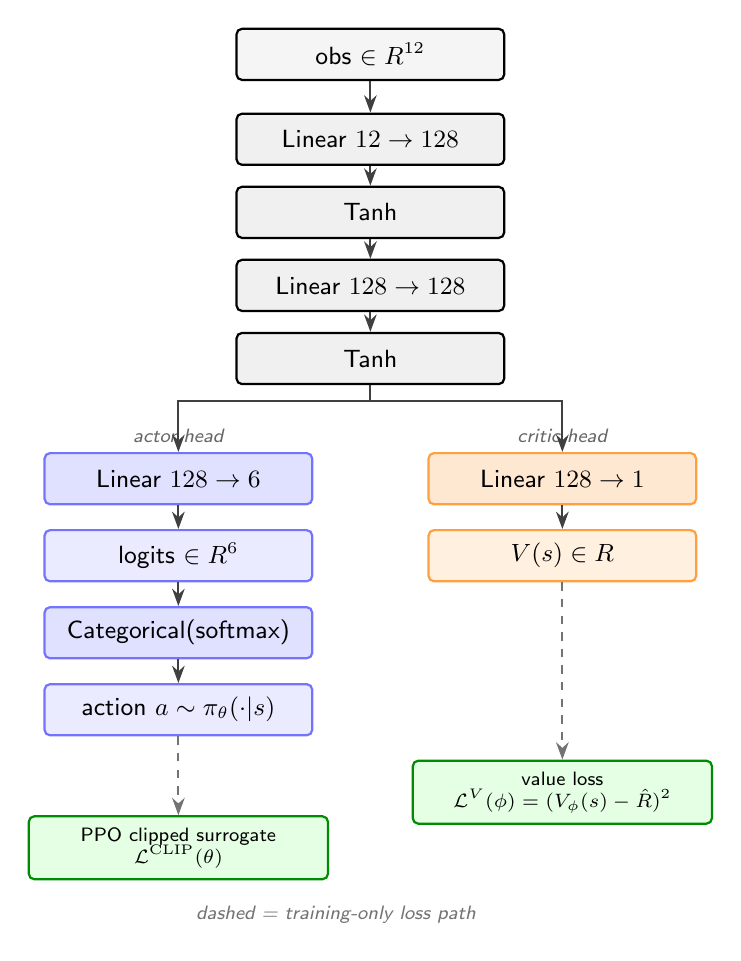
\begin{tikzpicture}[
  font=\sffamily\small,
  >={Stealth[length=2.2mm,width=1.6mm]},
  layer/.style={
    draw, rounded corners=2pt, thick,
    minimum width=34mm, minimum height=6.5mm,
    align=center, fill=gray!10
  },
  trunk/.style={layer, fill=gray!12},
  alayer/.style={layer, fill=blue!12, draw=blue!55},
  clayer/.style={layer, fill=orange!18, draw=orange!75},
  io/.style={
    draw, thick, rounded corners=2pt,
    minimum width=34mm, minimum height=6.5mm,
    align=center, fill=black!4
  },
  loss/.style={
    draw, rounded corners=2pt, thick,
    minimum width=38mm, minimum height=8mm,
    align=center, fill=green!10, draw=green!55!black,
    font=\sffamily\scriptsize
  },
  arr/.style={->, thick, draw=black!75},
  branchlbl/.style={font=\sffamily\scriptsize\itshape, text=black!60},
  dashedarr/.style={->, thick, draw=black!55, dashed}
]

% ---- input ----
\node[io] (in) {obs $\in \mathbb{R}^{12}$};

% ---- shared trunk ----
\node[trunk, below=4mm of in]      (fc1)  {Linear $12 \to 128$};
\node[trunk, below=2.5mm of fc1]   (th1)  {Tanh};
\node[trunk, below=2.5mm of th1]   (fc2)  {Linear $128 \to 128$};
\node[trunk, below=2.5mm of fc2]   (th2)  {Tanh};

% ---- split anchor ----
\node[below=4mm of th2] (split) {};

% ---- actor head (left, blue) ----
\node[alayer, below left=2mm and 6mm of split] (afc)   {Linear $128 \to 6$};
\node[io,    below=3mm of afc,
       fill=blue!8, draw=blue!55]               (alog)  {logits $\in \mathbb{R}^{6}$};
\node[alayer, below=3mm of alog]                (acat)  {Categorical(softmax)};
\node[io,    below=3mm of acat,
       fill=blue!8, draw=blue!55]               (aact)  {action $a \sim \pi_{\theta}(\cdot|s)$};

% ---- critic head (right, orange) ----
\node[clayer, below right=2mm and 6mm of split] (cfc)   {Linear $128 \to 1$};
\node[io,    below=3mm of cfc,
       fill=orange!12, draw=orange!75]          (vout)  {$V(s) \in \mathbb{R}$};

% ---- branch labels ----
\node[branchlbl, above=0pt of afc] {actor head};
\node[branchlbl, above=0pt of cfc] {critic head};

% ---- losses (training-only) ----
\node[loss, below=10mm of aact]
   (lpi)
   {PPO clipped surrogate\\$\mathcal{L}^{\mathrm{CLIP}}(\theta)$};
\node[loss, below=10mm of vout, yshift=-12.5mm]
   (lv)
   {value loss\\$\mathcal{L}^{V}(\phi) = (V_{\phi}(s)-\hat{R})^{2}$};

% ---- arrows: trunk ----
\draw[arr] (in)  -- (fc1);
\draw[arr] (fc1) -- (th1);
\draw[arr] (th1) -- (fc2);
\draw[arr] (fc2) -- (th2);

% split into two heads
\draw[arr] (th2.south) -- ++(0,-2mm) -| (afc.north);
\draw[arr] (th2.south) -- ++(0,-2mm) -| (cfc.north);

% actor chain
\draw[arr] (afc)  -- (alog);
\draw[arr] (alog) -- (acat);
\draw[arr] (acat) -- (aact);

% critic chain
\draw[arr] (cfc)  -- (vout);

% feed into losses (training-time)
\draw[dashedarr] (aact.south) -- (lpi.north);
\draw[dashedarr] (vout.south) -- (lv.north);

% legend / training-only note
\node[font=\sffamily\scriptsize\itshape, text=black!55,
      below=2mm of lpi, xshift=20mm]
  {dashed = training-only loss path};

\end{tikzpicture}
\end{document}
